\documentclass{article}
\usepackage{graphicx}
\usepackage{booktabs}
\usepackage{geometry}
\usepackage{tikz}
\usetikzlibrary{shapes, arrows.meta, positioning, backgrounds, fit}

\geometry{a4paper, margin=1in}

\title{Intelligent EV Charging Demand Prediction \\ \large Milestone 1: Model Evaluation \& System Architecture}
\author{Project 15 \\ \textbf{Batch: Section - C}}
\date{February 16, 2026}

\begin{document}

\maketitle

\section{Executive Summary}
This report analyzes the performance of the Machine Learning model developed to predict EV charging station utilization rates. The model uses historical usage data along with temporal, environmental, and traffic features to forecast demand.

\section{Problem Statement}
The rapid adoption of electric vehicles (EVs) has created significant challenges for power grid management and infrastructure planning. Charging stations often experience unpredictable surges in demand, leading to grid instability or long wait times for users. There is a critical need for an intelligent system that can accurately forecast charging station utilization based on multi-modal data (temporal, weather, and traffic) to optimize resource allocation and enhance user experience.

\textbf{Key Results:}
\begin{itemize}
    \item \textbf{R-Squared ($R^2$):} 0.9045 (Excellent predictive power)
    \item \textbf{RMSE:} 0.0926 (Low average error magnitude)
    \item \textbf{MAE:} 0.0634 (Very low absolute error)
\end{itemize}

The model demonstrates strong capability in conducting accurate demand forecasting, suitable for infrastructure planning and real-time user insights.

\section{System Architecture}

\begin{figure}[h]
    \centering
    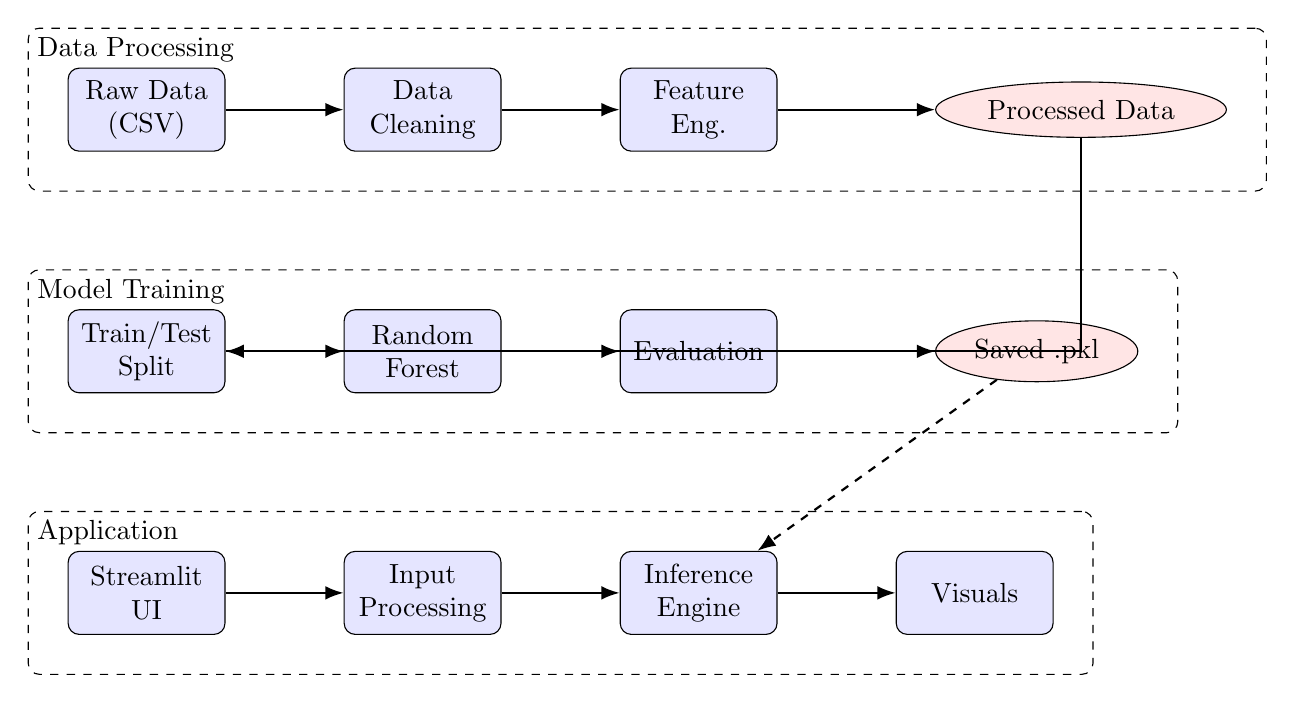
\begin{tikzpicture}[
        node distance=1.5cm,
        auto,
        block/.style={rectangle, draw, fill=blue!10, text width=5em, text centered, rounded corners, minimum height=3em},
        cloud/.style={draw, ellipse, fill=red!10, node distance=2cm, minimum height=2em},
        decision/.style={diamond, draw, fill=green!10, text width=4.5em, text bad centered, inner sep=0pt},
        line/.style={draw, -Latex, thick},
        container/.style={draw, dashed, inner sep=0.5cm, rounded corners, label={[anchor=north west]north west:#1}}
    ]
        % Data Layer
        \node [block] (raw) {Raw Data (CSV)};
        \node [block, right=of raw] (clean) {Data Cleaning};
        \node [block, right=of clean] (feat) {Feature Eng.};
        \node [cloud, right=of feat] (processed) {Processed Data};
        
        \path [line] (raw) -- (clean);
        \path [line] (clean) -- (feat);
        \path [line] (feat) -- (processed);
        
        \begin{scope}[on background layer]
            \node [container=Data Processing, fit=(raw) (processed)] (data_layer) {};
        \end{scope}

        % Model Layer
        \node [block, below=2cm of raw] (split) {Train/Test Split};
        \node [block, right=of split] (rf) {Random Forest};
        \node [block, right=of rf] (eval) {Evaluation};
        \node [cloud, right=of eval] (model) {Saved .pkl};

        \path [line] (processed) |- (split); % Link from Data to Model
        \path [line] (split) -- (rf);
        \path [line] (rf) -- (eval);
        \path [line] (eval) -- (model);
        
        \begin{scope}[on background layer]
            \node [container=Model Training, fit=(split) (model)] (model_layer) {};
        \end{scope}

        % Application Layer
        \node [block, below=2cm of split] (ui) {Streamlit UI};
        \node [block, right=of ui] (input) {Input Processing};
        \node [block, right=of input] (infer) {Inference Engine};
        \node [block, right=of infer] (viz) {Visuals};

        \path [line] (ui) -- (input);
        \path [line] (input) -- (infer);
        \path [line] (infer) -- (viz);
        \path [line, dashed] (model) -- (infer); % Link from Model to App

        \begin{scope}[on background layer]
            \node [container=Application, fit=(ui) (viz)] (app_layer) {};
        \end{scope}

    \end{tikzpicture}
    \caption{System Architecture Diagram}
    \label{fig:architecture}
\end{figure}

\section{Model Specification}
\begin{itemize}
    \item \textbf{Algorithm:} Random Forest Regressor
    \item \textbf{Framework:} Scikit-Learn (Pipeline with ColumnTransformer)
    \item \textbf{Input Features:}
    \begin{itemize}
        \item \textbf{Temporal:} Hour of Day, Day of Week, Is Weekend, Is Peak Hour
        \item \textbf{Environmental:} Temperature (°F), Precipitation (mm), Weather Category
        \item \textbf{Contextual:} Traffic Congestion Index, Gas Price, Local Events
        \item \textbf{Station:} Location Type, Charger Type, City
    \end{itemize}
\end{itemize}

\section{Data Description \& EDA Process}
\subsection{Data Sources \& Features}
The dataset is derived from historical EV charging session logs, capturing diverse operational environments across multiple urban centers. It includes over 5,000 sessions with granular data point frequency. Key features include:
\begin{itemize}
    \item \textbf{Temporal:} Timestamp (converted to seasonal context), Hour of Day, Day of Week, Is Weekend, Is Peak Hour.
    \item \textbf{Environmental \& Contextual:} Real-time temperature, precipitation levels, Traffic Congestion Index (scaled 1-3), historical gas prices, and boolean flags for local community events.
    \item \textbf{Station-Specific:} Location Type (Public/Residential/Commercial), Charger Type (Level 1/2/DC Fast), and City context.
\end{itemize}
The target variable is the \textbf{Utilization Rate (\%)}, representing the ratio of active charging sessions to total available port capacity at a given timestamp.

\subsection{Exploratory Data Analysis (EDA) Insights}
During the EDA phase, several critical correlational thresholds were established:
\begin{itemize}
    \item \textbf{Temporal Surges:} Utilization spikes sharply during established peak hours (7-10 AM and 4-7 PM), confirming commuter charging dominance.
    \item \textbf{Traffic Correlation:} A strong positive correlation exists between the Traffic Congestion Index and charging demand at urban stations.
    \item \textbf{Weather Impact:} Extreme weather conditions marginally increase utilization variance, likely due to battery efficiency drops forcing unexpected charging stops.
\end{itemize}

\section{Methodology \& Optimization}
\subsection{Design Justification}
A \textbf{Random Forest Regressor} was selected over simpler linear models due to its ability to capture non-linear interactions (e.g., the combined effect of high traffic \textit{and} bad weather). It was also chosen over Deep Learning approaches to align with Milestone 1 constraints prioritizing classical Machine Learning and interpretability.

\subsection{Optimization Steps}
To improve model performance, the following optimization steps were taken:
\begin{enumerate}
    \item \textbf{Feature Engineering:} Redundant features (like engineered `is_rush_hour` when `is_peak_hour` existed) were stripped to reduce dimensionality.
    \item \textbf{Pipeline Architecture:} Constructed a scikit-learn \texttt{ColumnTransformer} pipeline. This ensures \texttt{StandardScaler} is isolated to numeric features and \texttt{OneHotEncoder} to categorical features, preventing data leakage during inference.
    \item \textbf{Hyperparameter Tuning:} Tree depth was restricted (\texttt{max\_depth=10}) and estimator count controlled (\texttt{n\_estimators=50}) to prevent overfitting and ensure the model artifact remained lightweight ($<3$MB) for agile deployment.
\end{enumerate}

\section{Detailed Performance Metrics}

\begin{table}[h]
    \centering
    \begin{tabular}{@{}llp{8cm}@{}}
        \toprule
        \textbf{Metric} & \textbf{Value} & \textbf{Interpretation} \\
        \midrule
        R-Squared ($R^2$) & 0.9045 & The model explains \textbf{90.45\%} of the variance in charging demand. Indicates high fit to real-world patterns. \\
        RMSE & 0.0926 & On average, predictions deviate by \textbf{9.3\%} from actual utilization. \\
        MAE & 0.0634 & The average absolute difference between predicted and actual utilization is \textbf{6.3\%}. \\
        \bottomrule
    \end{tabular}
    \caption{Model Evaluation Metrics}
    \label{tab:metrics}
\end{table}

\section{Team Contribution}
\begin{itemize}
    \item \textbf{Sachin Jaiswal:} Core Machine Learning model development, pipeline architecture, and training.
    \item \textbf{Ayush Tiwari:} Data cleaning infrastructure, preprocessing logic, and presentation design.
    \item \textbf{Sibtain Ahmed Qureshi:} Technical report drafting, LaTeX documentation, and data quality assurance.
    \item \textbf{Md. Sajjan:} Frontend UI development, Streamlit dashboard implementation, and custom styling.
\end{itemize}

\section{Conclusion}
The Random Forest model satisfies the technical requirements for Milestone 1, achieving high accuracy via classical optimization techniques. It operates effectively within an interactive Streamlit framework, establishing a solid baseline before advancing to Agentic AI infrastructure planning.

\end{document}
